
\begin{frame}{Conception des Portes logiques : plusieurs niveaux d'abstraction}
  [Guyot TIMA 1995]
  \begin{center}
    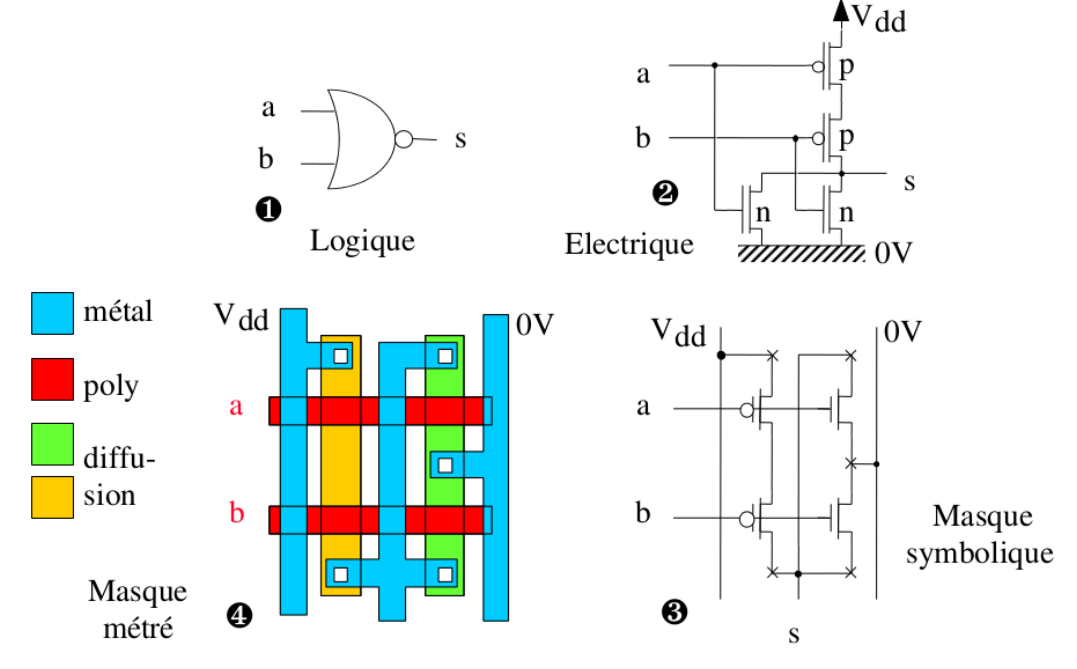
\includegraphics[scale=0.3]{./images/guyot.png}
  \end{center}
\end{frame}


\begin{frame}{Conception des Systèmes numériques : Y de Gajski}

  \begin{columns}[T,onlytextwidth]
    \begin{column}{0.47\textwidth}
      \begin{center}
        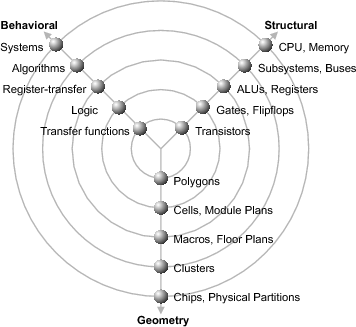
\includegraphics[scale=0.4]{./images/y_gajski.png}
        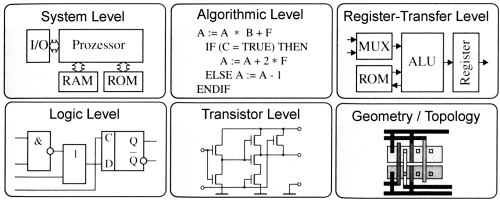
\includegraphics[scale=0.3]{./images/y_gajski_2.png}
      \end{center}
    \end{column}

    \begin{column}{0.51\textwidth}
      \begin{center}
        \includegraphics[scale=0.15]{./images/gajski.jpg}
        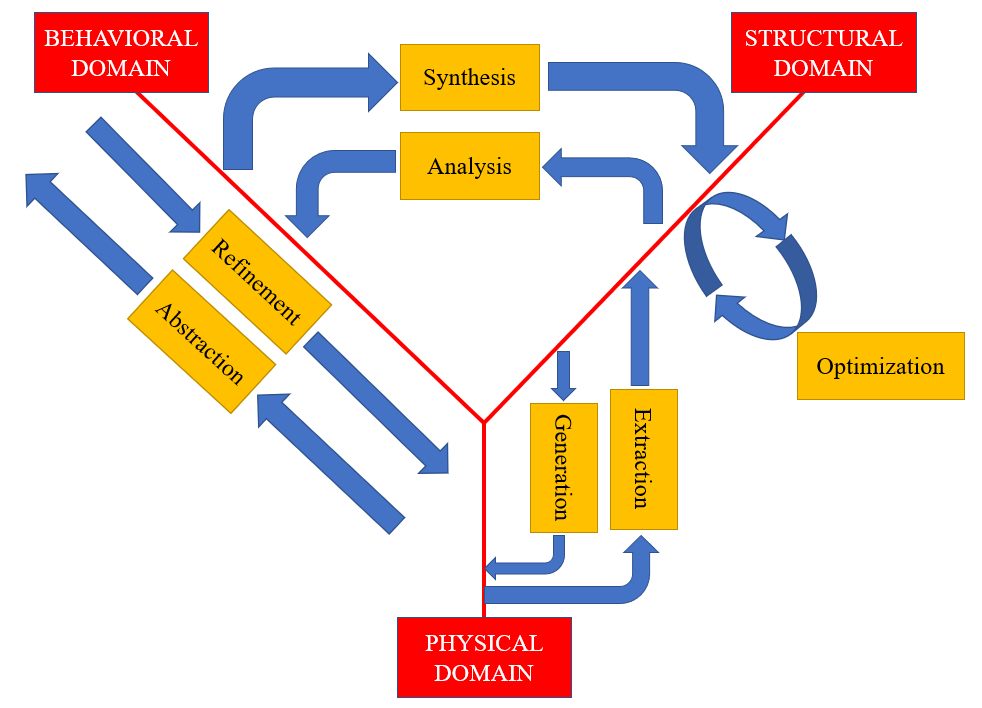
\includegraphics[scale=0.30]{./images/y_gajski_3.png}
      \end{center}
    \end{column}
  \end{columns}

\end{frame}

\begin{frame}{Abstraction et Synthèse automatique}
  \begin{columns}
    \begin{column}{0.50\textwidth}
      \begin{itemize}
        \item Complexité des systèmes
        \item Recours à des langages spécifiques : HDL.
        \begin{itemize}
          \item Description
          \item Simulation (laboratoire virtuel)
          \item Synthèse automatique
        \end{itemize}
        \item ...à différents niveaux d'abstraction.
      \end{itemize}
    \end{column}
    \begin{column}{0.50\textwidth}
      \begin{center}
        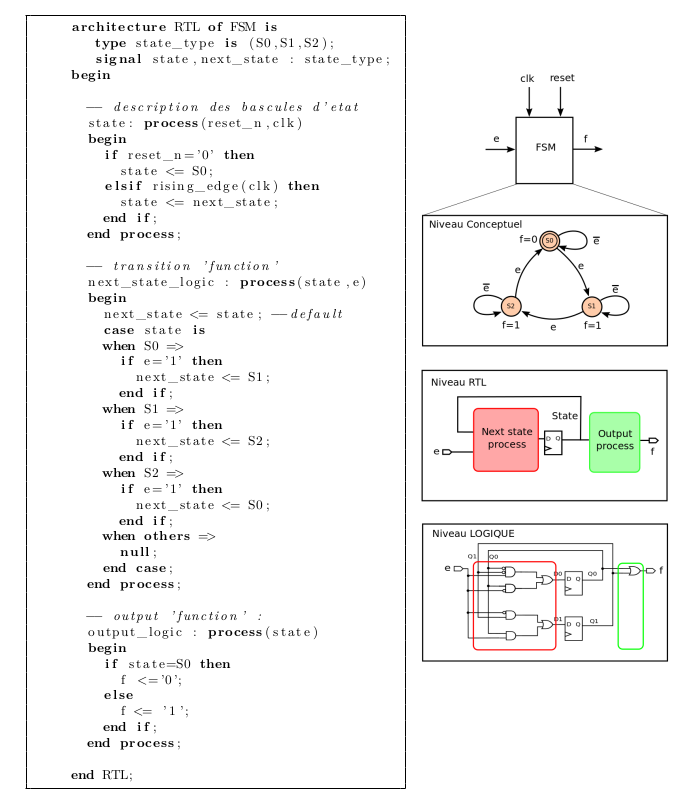
\includegraphics[scale=0.25]{./images/fsm.png}
      \end{center}
    \end{column}
  \end{columns}
\end{frame}

\begin{frame}{Abstractions : système et automates}
  \begin{center}
    \includegraphics[scale=1.0]{./images/gemini_abstraction_soc.jpeg}
  \end{center}
\end{frame}
